\section{Integration und Programmierung der Steuerungstechnik \textcolor{gray}{ (Vincent Sonvilla)}}


\subsection{Aufgabenstellung}

\subsection{Tia-Portal Grundlagen}

Tia Portal (Totally Integrated Automation Portal) ist die zentrale Software von Siemens zur Programmierung, Konfiguration und Diagnose von Automatisierungssystemen. Es ermöglicht die Steuerung von SPS (Speicherprogrammierbare Steuerungen), HMI (Bedienpanels) und Antrieben in einer einzigen Umgebung.

    \subsubsection{Allgemeines}

        \paragraph{Arbeitsweise einer SPS} \mbox{} \\
        Eine SPS arbeitet zyklisch. In Abb. \ref{Arbeitsweise_einer_SPS} wird gezeigt wie ein solcher Zyklus aussieht. Bei erstmaligem Starten oder Neustarten der SPS werden zuerst alle Ausgänge, Merker, etc. auf Null gesetzt. Danach startet die zyklische Arbeitsweise. Zuerst wird ein Prozessabbild der Eingänge gemacht. Mit diesen Eingangswerten wird dann das Programm ausgeführt. Anschließend wird ein Prozessabbild der Ausgänge gemacht. Dieses wird dann an die Ausgänge übergeben. Danach beginnt der Zyklus von vorne. \cite{Arbeitsweise_der_SPS}
        \begin{figure}[h]
            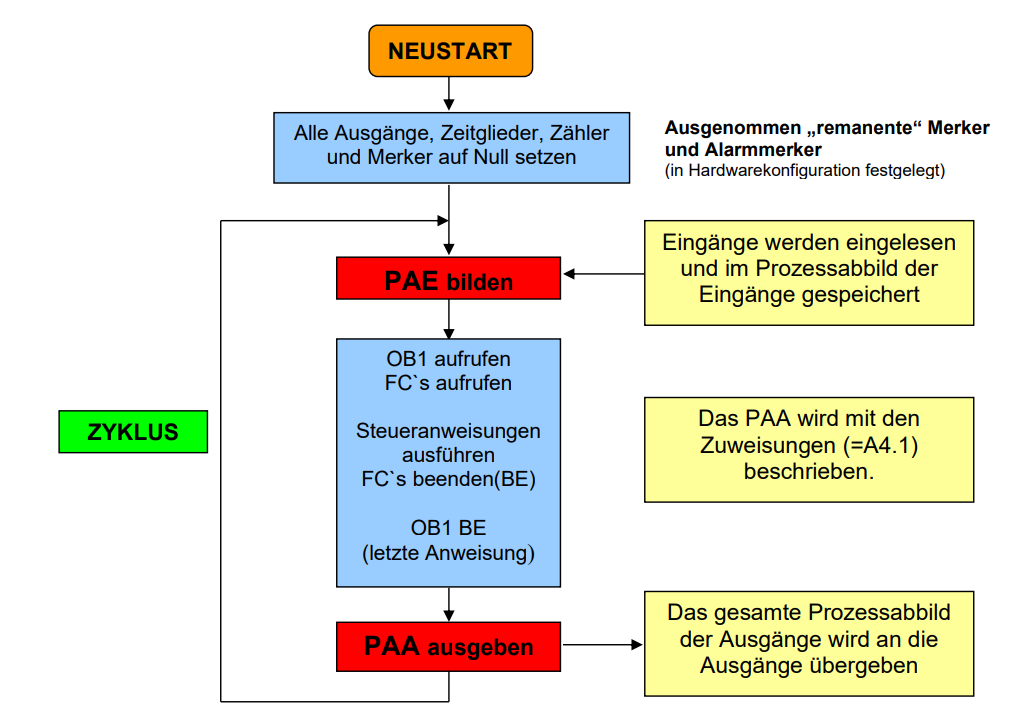
\includegraphics[width=0.9\textwidth]{Sonne/Arbeitsweise_einer_SPS.png}
            \caption{Arbeitsweise einer SPS \cite{Arbeitsweise_der_SPS}}
            \label{Arbeitsweise_einer_SPS}
        \end{figure}

        noch Datentypen, ... maybe

    \subsubsection{Programmbausteine}
    
    In TIA Portal werden Programmbausteine genutzt, um Steuerungsprogramme modular und strukturiert zu gestalten. Dadurch werden Programme übersichtlicher, wiederverwendbar und effizienter. Es gibt unterschiedliche Arten von Programmierbausteinen:

    \begin{itemize}
        \item[1.] \textbf{OB(Organisationsbausteine)} \\
            Organisationsbausteine werden verwendet um das Anwenderprogramm hierarchisch zu strukturieren. Auch für OBs stehen,wie in Abb. \ref{Organisationsbausteine} gezeigt, unterchiedliche Bausteine zur Verfügung:
            \begin{figure}[h]
                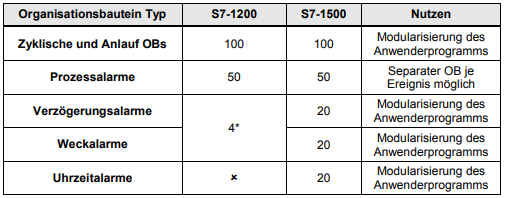
\includegraphics[width=\textwidth]{Sonne/Tia-Portal_Organisationsbausteine.png}
                \caption{Organisationsbausteine \cite{Programmierleitfaden_für_S7-1500}}
                \label{Organisationsbausteine}
            \end{figure}

            Organisationsbausteine steuern unterschidiedliche Vorgänge:
            \begin{itemize}
                \item Anlaufverhalten der Steuerung
                \item Zyklische Programmbearbeitung
                \item Alarmgesteuerte Programmbearbeitung
                \item Behandlung von Fehlern
            \end{itemize}
            Werden in einem Programm mehrere OBs aufgerufen, so werden die OBs in aufsteigender Reihenfolge der OB-Nummer abgearbeitet. 
            \cite{Programmierleitfaden_für_S7-1500}

        \item[2.] \textbf{FC(Funktionen)} \\
            Funktion haben keinen zyklischen Datenspeicher, deswegen können Bausteinparameter nicht bis zum nächsten Aufruf gespeichert werden. Darum müssen Funktionen bei jedem Aufruf mit Aktualparametern versorgt werden. Um kein zufälliges Verhalten enstehen zu lassen sind die Werte immer mit einem Defaultwert vorbelegt. Will man die Daten einer Funktion dauerhaft speichern, so muss man einen globalen Datenbaustein verwenden.\\
            Funktionen werden verwendet, um häufig wiederkehrende Anwendungen durchzuführen.
            \cite{Programmierleitfaden_für_S7-1500}
            
        \item[3.] \textbf{FB(Funktionsbausteine)} \\
            Im Gegensatz zu Funktionen haben Funktionsbausteine einen zyklischen Datenspeicher -Instanz DB-, in welchem Werte dauerhaft gespiechert werden.Dadurch behalten statische Variablen ihren Wert von Zyklus zu Zyklus. Wie bei Funktionen sind die Werte mit einem Defaultwert vorbelegt.\\
            Funktionsbausteine können genutzt werden, um Unterprogramme für unterschiedliche Anwendungen zu erstellen. Außerdem werden sie genutzt um das Anwenderprogramm zu strukturieren. Bei mehrfacher Verwendung von Funktionsbausteinen empfiehlt sich die Verwendung von Multiinstanz-DBs.
            \cite{Programmierleitfaden_für_S7-1500}
        
        \item[4.] \textbf{Global-DB(Datenbausteine)} \\
            Globale Datenbausteine speichern variable Daten, die dem kompletten Programm zur Verfügung stehen. Wie in Abb.\ref{Zugriff auf Global-DB} ersichtlich, bedeutet das ,dass alle Bausteine Zugriff auf den Global-DB haben.

            \begin{figure}[h]
                \centering
                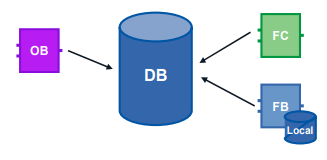
\includegraphics{Sonne/Zugriff_auf_Global-DBs.png}
                \caption{Zugriff auf Global-DB \cite{Programmierleitfaden_für_S7-1500}}
                \label{Zugriff auf Global-DB}
            \end{figure}

            In Globalen Datanbausteinen können jegliche Datentypen genutzt werden.\\
            Globale DBs werden verwendet, wenn Daten in verschiedenen Programmteilen bzw. Bausteinen benötigt werden.
            \cite{Programmierleitfaden_für_S7-1500}

        \item[5.] \textbf{Instanzen} \\
            Wird ein Funktionsbaustein aufgerufen, so nennt man das Instanz. Die Daten der Instanz, werden im sogenannten Instanzdatenbaustein gespeichert. Instanz-DBs werden automatisch nach den Vorgaben des Funktionsbausteins erzeugt und können somit nicht direkt geändert werden. Der Instanz-DB hat einen dauerhaften Speicher, welcher die Schnittstellen Input, Output, InOut sowie Static beihaltet. Zusätzlich besitzt der Instanz-DB einen flüchtigen Datenspeicher in dem tempöräre Variablen gespeichert werden. Diese sind dadurch immer nur für einen Zyklus gültig.
            
        \item[6.] \textbf{Multiinstanzen} \\
            Bei Multiinstanzen speichert der Funktionsbausetein seine Daten in den Instanz-DB des übergeordneten Funktionsbaustein. Das heißt es wird in einem FB ein anderer FB aufgerufen. Dieser speichert seine Daten dann im Instanz-Db des Funktionsbausteins, welcher ihn aufgerufen hat. Multiinstanzen helfen das Programm übersichtlicher sowie strukturierter zu halten, da man mehrere Instanzen in einer Instanz vereint.

    \end{itemize}

    \subsubsection{Technologieobjekte}
    Technologieobjekte dienen dazu die Ansteuerung und Handhabung von technischen Funktionen, insbesondere von Motoren, Achsen, etc. zu vereinfachen. Es existieren eine Vielzahl an unterschiedlichen Technologieobjekten. In nachfolgenden Absätzen werden die für das Projekt relevanten Technologieobjekte genauer erklärt.

    \begin{itemize}

        \item[1.] \textbf{Positionierachse (PositioningAxis)} \\
            Dieses Technologieobjekt dienz zur genauen Positionierung einer Achse, sowie der Rückmeldung der aktuellen Achsposition. Zusätzlich wird die Zielposition automatisch gehalten. \\
            Für die Positionierachse stehen folgende Motion Control Anweisungen zur Verfügung: 
            \begin{itemize}
                \item Home \\
                    Aktives oder passives Referenzieren der Achse.
                \item MoveAbsolut \\
                    Fahren der Achse auf eine absolute Position.
                \item MoveRelativ \\
                    Fahren der Achse auf eine Position relativ zur aktuellen Position.
                \item MoveSuperimposed \\
                    Starten einer überlagerten Bewegung zu einer bereits laufenden Bewegung.
                \item TorqueLimiting \\
                    Aktivieren einer Momentbegrenzung oder Festanschlagserkennung.
                \item SetSensor \\
                    Umschalten des Gebers für die Achse. 
                    \cite{Technologieobjekte}
            \end{itemize}
            

        \item[2.] \textbf{Gleichlaufachse (SynchronousAxis)} \\
            Das Technologieobjekt Gleichlaufachse enthält alle Funktionen des Technologieobjekts Positionierachse. Zusätzlich lässt sich die Achse mit einer Leitachse verschalten, sodass diese der Positionsänderung der Leitachse folgt. Dieses Technologieobjekt wird verwendet um synchrone bzw. positionsabhängige Bearbeitungsvorgänge auszuführen. \\
            Der Gleichlaufachse stehen folgende zusätzliche Motion Control Anweisungen zur Verfügung:
            \begin{itemize}
                \item GearIn \\
                    Starten eines relativen Gleichlaufs einer Leit- und Fogeachse.
                \item GearInPos \\
                    Starten eines absoluten Gleichlaufs einer Leit- und Fogeachse unter Vorgabe einer Synchronposition.
                \item PhasingAbsolut \\
                    Absolutes Verschieben des Leitwertbeugs whärend eines aktiven Gleichlaufs.
                \item PhasingRelativ \\
                    Relatives Verschieben des Leitwertbeugs whärend eines aktiven Gleichlaufs.
                \item CamIn \\
                    Start eines absoluten Kurvenscheibengleichlaufs.
                \item SynchronizedMotionSimulation \\
                    Simulation eines aktiven Gleichlaufs. 
                    \cite{Technologieobjekte}
            \end{itemize}
             
    \end{itemize}

    \subsubsection{Programmiersprachen}
    In Tia Portal stehen unterschidiedliche Programmiersprachen zu Verfügung. Je nach Präferenz bzw. Aufgabe ist das Nutzen der richtigen Sprache von Vorteil. Daher folgt hier eine Auflistung der möglichen Programmiersprachen, welche sich in textbasierte oder graphische Sprachen unterteilen. 

    \begin{itemize}
        \item [1.] \textbf{Funktionsplan(FUP) - Funktion Block Diagramm(FDP)} \\
            FUP ist eine graphisch augebaute Programmiersprache. Sie besteht aus unterschiedlichen Bausteinen, in Blockdarstellung, welche graphisch durch Linien verknüpft werden. Die Signalverarbeitung bei FUP läuft von links nach rechts. Die Programmierlogik in FUP ist übersichtlich und schnell nachzuvollziehen, weswegen diese Sprache für Anfänger relativ gut geeignet ist. 
            \cite{Programmiersprachen_der_SPS}

        \item[2.] \textbf{Kontaktplan(KOP) - Ladder Diagram(LD)} \\
            Der Kontakplan ähnelt einem Stromlaufplan, der anstatt von oben nach unten von links nach rechts verläuft. Für die Programmierung werden Symoble wie Öffner, Schließer und Ausgänge verwendet. Da nicht für jeden Baustein ein Symbol verfügbar ist, werden solche Bausteine in FUP dargestellt. Der logische Verlauf der Schaltung ist dabei von links nach rechts und von oben nach unten.
            \cite{Programmiersprachen_der_SPS}

        \item[3.] \textbf{Anweisungsliste(AWL)} \\
            AWL ist eine textbasierte Programmiersprache, welche an Assembler angelehnt ist. Die Programmiersprache AWL wird hauptsächlich zur logischen Verknüpfung von Ein- und Ausgängen verwendet.In AWL werden Anweisungen in der Reihenfolge geschrieben, in der sie ausgeführt werden sollen. Da AWL für die Programmierung von größeren Projekten eher ungeeignet ist, wird es in neueren Programmen immer weniger verwendet.
            \cite{Anweisungsliste}


    \end{itemize}


    \subsubsection{Bilbliotheken}
    \label{Bibliotheken}


\subsection{Motorenansteuerung}

\subsection{SPS-Server Kommunikation}

    \subsubsection{Zur Auswahl stehende Kommunikationsprotokolle} 
    \label{Kommunikationsprotokolle}

    Kommunikationsprotokolle ermöglichen den Datenaustausch zwischen unterschiedlichen Systemen, indem sie Standards und Regeln für die Kommunikation definieren. In diesem Projekt wurden zwei Protokolle getestet und miteinander verglichen: OPC-UA sowie das HTTP-Protokoll.


         \paragraph{Allgemeines}

        \begin{itemize}
            \item \textbf{HTTP (Hypertext Transfer Protocol):}  \mbox{} \\
            HTTP ist eines der bekanntesten Protokolle, welches für die Datenübertragung zwischen Clients und Servern verwendet wird. Es basiert auf einem Anforderungs-Antwort-Prinzip, bei dem ein Client (Bsp.: Webbrowser) Anfragen an einen Server sendet, welcher anschließend die entsprechenden Daten zurückschickt. Die Anfrage wird als HTTP Request und die Antwort als HTTP Response bezeichnet.\cite{HTTP-Allgemein}
            
            \item \textbf{OPC-UA (Open Platform Communications - Unified Architecture):} \mbox{} \\
            OPC-UA (Open Platform Communications Unified Architecture) ist ein plattformunabhängiges Kommunikationsprotokoll, das speziell für industrielle Anwendungen entwickelt wurde. Es ermöglicht eine herstellerunabhängige Kommunikation zwischen verschiedenen Geräten bzw. Systemen. \cite{OPC-UA}
        \end{itemize}

        \paragraph{Funktionsweise}

            \begin{itemize}
                \item \textbf{{HTTP (Hypertext Transfer Protocol):}} \mbox{} \\
                
            
                \item \textbf{{OPC-UA (Open Platform Communications - Unified Architecture):}} \mbox{} \\
                
            \end{itemize}
        
            

    
    \subsubsection{Verbindungsherstellung}
    Aus den in Punkt \ref{Kommunikationsprotokolle} genannten Gründen wurde das HTTP Protokoll ausgewählt. Um in TIA-Portal die Verbindung via HTTP aufzubauen, benötigt man bestimmte Libraries die von Siemens zu Verfügung gestellt werden. Diese müssen dann wie im Punkt \ref{Bibliotheken} gezeigt eingebunden werden, um die Funktionsbausteine der Library nutzen zu können. 

        \paragraph{Funktionsbausteine} \mbox{} \\
        In der Library stehen dann folgende Bausteine zur Verfügung:

        \begin{itemize}
            \item GET
            \item POST-PUT \\
            Mit dem POST-PUT Befehl werden Daten zum Server geschickt aber auch Daten erhalten. 
        \end{itemize}


    \subsubsection{Datenfilterung}
    Die vom Server geschickten Daten werden in einem Befehl geschickt. Aus diesem Befehl muss herausgelesen werden um welche Aufgabe es sich handelt, und die Daten die erforderlich sind um diesen Befehl auszuführen.

        \paragraph{Datenformatierung}\mbox{}\\
        Die Daten werden in einem String geschickt, welcher in zwei Teile aufgeteilt wird. Der zweite Teil ist jedoch abhängig vom ersten. \\
        
        \begin{itemize}
            \item 1.Teil: \\
            IDXXXXAXX \\
            Aus diesem Teil werden die ID-Nummer sowie der Auftrag herausgefiltert. Die ID-Nummer ist eine 4 stellige Nummer welche nach ID steht. Der Auftrag welcher ausgeführt werden muss steht in den zwei Stellen nach A.\\
            Diese werden nach folgender Codierung ausgelesen:
                \subitem 00: Kommissionierstation
                \subitem 01: Förderband
                \subitem 10: Lager 1 (Aus-/Einlagerung)
                \subitem 11: Lager 1 (Querförderer)
            \item 2.Teil: \\
            Der zweite Teil steht in Abhängigkeit zu ersten. Je nachdem welche Zahl nach A steht,also der Code welche Area angesprochen wird, ist der zweite Teil anders aufgebaut.
                \begin{itemize}
                \item 00: 
                \item 01:
                \item{10: X-Position, Y-Position, Z-Position,Ein/-Auslagerung \\
                Wobei nach jedem Symbol eine 4 stellige Zahl steht.Also X0000Y0000Z0000R0 bedeutet, dass die 
                X-Position 0, Y-Position 0, Z-Position 0 und es sich um eine Auslagerung handelt.}
                \item 11:
                
                \end{itemize}
            
        \end{itemize}

\subsection{Herausforderungen}
